%last updated in April 2002 by Antje Endemann

\documentclass[runningheads]{llncs}
%In order to omit page numbers and running heads
%please use the following line instead of the first command line:
%\documentclass{llncs}.
%Furthermore change the line \pagestyle{headings} to
%\pagestyle{empty}.

\usepackage[pdftex]{graphicx}
% declare the path(s) where your graphic files are
\graphicspath{{./figures/}}
% and their extensions so you won't have to specify these with
% every instance of \includegraphics
\DeclareGraphicsExtensions{.eps,.pdf,.png}

\usepackage[cmex10]{amsmath}
\usepackage{mathrsfs}
\usepackage{amsfonts}
\usepackage{multirow}

\def\x{{\mathbf x}}
\def\L{{\cal L}}
\def\S{{\cal S}}
\def\N{{\cal N}}
\def\A{{\mathbf A}}
\def\B{{\mathbf B}}
\def\M{{\cal M}}

\input{psfig.sty}

\begin{document}

\pagestyle{headings}
%In order to omit page numbers and running heads
%please change this line to
%\pagestyle{empty}
%and change the first command line too, see above.

\mainmatter

\title{Feature evaluation in handwritten characters for regressive and generative Hidden Markov Models}

\titlerunning{Lecture Notes in Computer Science}

\maketitle

\begin{abstract}
Hidden Markov Model has been an established method often employed for handwritten character recognition. The current work aims at evaluating some of the feature extraction procedures in the character recognition literature that are frequently used in a common Hidden Markov Model framework. This should facilitate better understanding of the features and also help capture the information that aids respective feature extractor in the classification task. The effects of model topologies and data normalization are also studied over different hand written data-sets. The Hidden Markov Model framework is then used to generate handwritten text to further evaluate the features.
\end{abstract}

\section{Introduction}
\label{sec:intro}
Transcription of digitized documents is an important task gaining lot of attention from the image processing and pattern recognition research community. Degradation of the documents over time, variation in the writing styles, inconsistent document background based on the medium are but a few challenges encountered when working in this field. One of the methods that has been successful in this area are the hidden Markov models (HMMs) \cite{Fink09} which are based on sound mathematical formulations. These models have their origin in speech recognition and are good at handling data sequences. Since text is often written along one direction, handling text as a sequence of characters fits well within the HMM paradigm.

Training for a finite set of states an HMM of \emph{first order} i.e. current state depends only on the previous state,  depends on computing a matrix of \emph{state transition probabilities} denoted by $\A$, a vector of \emph{start probabilities} denoted by $\pi$, matrix of state specific \emph{output probabilities} distributions denoted by $\B$ and involves updating them with every relevant training example \cite{Rabi89}. In the current context we investigate into Baum-Welch and Bakis algorithms discussed in \cite{Rabi89}. The Baum-Welch algorithm is an Expectation-Maximization procedure that tries to answer question of determining the $(\pi, \A, \B)$ parameters which, help maximizing the HMM performance in an \emph{ergodic} or a \emph{fully connected} topology where every state is connected to every other state. However, there is an inherent directionality in Latin based text which, is exploited in the \emph{left-right} topology using Bakis algorithm, here the states move left to right but not the other way around further details on HMM implementation can be found in \cite{Rabi89}.

As HMMs are efficient at handling sequential information, images are often processed using a sliding window. The sliding window approach can be used at word or character level to identify words or characters respectively \cite{Fink09}. In the current approach the content within the sliding windows are used to extract features, which are then labeled. By concatenating labels, of successive sliding windows a string is formed corresponding to the image. A HMM-bank containing multiple HMMS is trained on the labeled training sequences, any query string is then classified based on a scoring mechanism over all the HMMs in the bank. This setup provides ideal testing environment to understand the strength of each feature when used along with an HMM. A Support Vector Machine (SVM) classifier is also trained on the features under study to provide a baseline for comparison.

This paper is structured into six sections where some background information has been provided in the introduction section. Insight into the HMM architecture used in the character classification is provided in the second section. The third section provides description of the features used in the training. Data-sets used in evaluating the features and the evaluation methodology is described in the fourth section followed by the results and conclusions.

\section{Hidden Markov Model Classifier}
\label{sec:HMM}
In order to evaluate various features we have followed a common pre-processing and classification stages for all the features. Each image is converted to a gray-scale image rescaled to $100 \times 100$ pixels. Binarization is carried out to aid in computing a specific aspect of the feature. The image is then divided into vertical non-overlapping segments, performance variation due to training an HMM on overlapping segments is not part of the current experimental setup. These image segment are then used to extract features. The features thus accumulated over the training data are then clustered and a label is assigned to each segment depending on the label of the respective centroid to which a feature vector belongs. The experiments are repeated with and without whitening the feature vector to understand its behavior.

A unique HMM is trained on the label string corresponding every processed character image. This approach results in an HMM-bank architecture with multiple HMMs where each HMM is trained for a unique character. The classification of a query image is done by converting it to a query string using the cluster centroids obtained from the training data, as the code book for a vector quantizer. The query string is then passed to each character HMM in the bank and likelihood score is returned. A decision based on the maximum score returned from HMM-bank results in the classification of the query image to a unique alphabet.\\

\subsection{HMM Architecture}
\label{ssec:archi}
In the current context HMMs are primarily used as classifiers of labeled sequences. In transcription of documents in Latin based script one is likely to encounter alphabet in both upper and lower case so an individual class for each character in each case is defined. This architecture leads to an HMM-bank with 52 individual HMMs, one for each character instance in upper and lower case. A special beginning and end states denoted by \textit{start} and \textit{end} respectively are introduced. In case the feature extraction step produces $n$ segments there will be $n + 2$ states in the HMMs. These special beginning and end states are included to facilitate concatenation multiple training observation sequences to form one observation sequence on which individual HMM is trained. In order to train an HMM a basic assumption on the topology is to be made based on application at hand. In transcription of document on Latin based scripts the left-right topology is a natural choice for the HMM topology \cite{Laan}. The initialization of the transition and emission matrices are done in such a way that the following properties are fulfilled:

\begin{itemize}
 \item Beginning and end states \textit{start}, \textit{stop} will always emit the special symbols @ and \$ respectively.
 \item The  \textit{start} state will always transit to the first normal state.
 \item The \textit{end} state always transits back to \textit{start}.
 \item The forward transition from all other states is to a state that has not been visited since the last visit to \textit{start}.
\end{itemize}

\subsection{Initial Parameter Selection}
\label{ssec:init}
There are many ways to generate an initial model, some techniques consider random initialization strategy which assigns the values in the transition and emission matrices to random values. In the count-based initialization for example the emission matrix is assigned based on frequency of labels from the training examples, the transition matrix however is assigned with uniform transition probability from current state to all reachable states. We have adopted the count based initialization for faster training of the HMMs \cite{Laan} though while the classification accuracy of both random and count-based initialization are similar.


\section{Feature Extraction}
\label{sec:feat}
In following section we provide a brief description of four feature extraction methods that are popular in character recognition. These features have been selected as they are well understood and are generic with good performance in character recognition.

\subsection{Naive Strip feature}
\label{ssec:nsf}
Each image is binarized and then divided into vertical segments. Within each segment connected components are identified and three of the maximal components are picked based on the component length, $C_l$. These components are then identified as long, $\L$ if $C_l \ge n\cdot w_d$, short, $\S$ if $w_d \le C_l < n \cdot w_d$, or none, $\N$ if $ C_l < w_d$, where $w_d$ is the width of the segment and $n$ is a scale-factor. We will end up in each segment identified with a triplet formed by $\L,\S,\N$. There can be 10 combinations of these triplets and these form the class labels for this feature. This feature is void of any need for clustering and has two parameters, number segments to divide the image into which determines the segment width $w_d$ and the other scale-factor $n$. In classical image processing ideology this approach though naive tries to identify the alphabets based on edge patterns in non-overlapping moving window  over an image  \cite{Cheriet}. The dimensionality of the resulting feature is equal to the number of segments the image was divided into.

\subsection{Marti-Bunke feature}
\label{ssec:mbf}
This is a nine dimensional feature that is obtained for each vertical segment of the image. This feature captures rough shape, texture and span information of each character by computing some statistics and estimates over each segment. The shape information is captured by computing the upper and lower contour position of the character in each segment, and the gradient of the upper and lower contours of the segment. The texture information is retained in the number of background-foreground transitions and by computing the number of foreground pixels between the  upper and lower contour divided by the height of the contour. The character span is estimated by computing mean, the center of gravity and the second order moment of the segment \cite{MartiBunke02}. For efficient computation of these features binarized as well as gray-scale images are required. This feature is compact representation of the shape information but lacks a scale estimate that is required in differentiating the upper and lower case alphabet for instance in the case  of \emph{x, o, c} etc.

\subsection{Gabor feature}
\label{ssec:gbf}
This feature can be seen as a counting metric that keeps track of the segments exceeding a certain threshold but takes both scale and the orientation into account when generating the overall feature. The feature is built by dividing the gray-scale image into a grid. A complex Gaussian kernel is built with varying sigma at different angles between the real and imaginary part of the kernel (the argument of a complex number) \cite{CCPBN10}. This builds up a series of Gaussian filters capturing various scales of interest controlled by the sigma of the Gaussian and at various angles controlled by the argument of the complex kernel. The mean of the absolute value of the convolution output is set as the threshold and the count of instances that have exceeded this threshold in each grid at each scale and orientation is cascaded to form the overall feature vector \cite{LKF05}. This feature is controlled by the scale, shape of the grid patches and the orientation parameters. The resulting feature vector is $n_s \cdot n_o \cdot n_g$ dimensional, where $n_s$ is the number of scales, $n_o$ is the number of orientations, $n_g$ is the number grid elements or the sub-images formed by the grid in the image. In the current framework five scales, eight orientations with twenty-five patches per image are the default parameter settings.

\subsection{Discrete Cosine Transform feature}
\label{ssec:dctf}
As in the case of Gabor feature we start by dividing the image into patches. Each patch is then subjected to a discrete cosine transform (DCT)  \cite{ANR74}. As most of the energy content of the image is contained in the low frequency, the coefficients are reordered by zig-zag scan in each patch. The most significant coefficients per patch can be picked up and cascaded to form the feature vector. The dimensionality in this case is $n_c \cdot n_g$, where $n_c$ is the number of significant coefficients, and $n_g$ is the number grid elements or the sub-images formed by the grid in the image \cite{ARJIA08}. In the default settings ten most significant coefficients over twenty-five patches are picked.

\section{Experiments}
\label{sec:exp}
The experiments conducted can be broadly classified in two categories. Firstly the regressive mode where a baseline is established against a well understood classifier in this case an SVM using a polynomial kernel of degree three. The focus has been on not only understanding the classification capability of the features but also capture the parameter settings that are well suited for each method such as effect of whitening and k-Means clusters which directly influence the number of labels at each state in the HMMs. These parameter settings are then used in the experiments where the HMMs are used as a generative models for characters in order to further understand the feature in capturing the variance in the handwriting over characters. In the experiments we perform an exhaustive search over features, evaluating effects of whitening, HMM topologies. We evaluate with two different kinds of data sets spanning both upper and lower case alphabet.

% -------------------------------------------------------------------------
\begin{figure}[t]

\begin{minipage}[b]{1.0\linewidth}
  \centering
  \centerline{\includegraphics[width=4.0cm,height=4.0cm]{data}}
%  \vspace{2.0cm}
%  \centerline{(a) Result 1}\medskip
\end{minipage}
\caption{Instances of 'a' in UniPenn(first row), NIST (second row)}
\label{fig:dataset}
%
\end{figure}

\subsection{Data-sets}
\label{ssec:data}
\subsubsection{UJIPenchar2}
The UniPenn2 dataset of online handwritten characters \cite{UJIPen} captures the stylus co-ordinates of 60 writers when writing two instances of each character in upper and lower case. This data-set has recorded information of 120 instances of each character as an (x,y)-coordinate trace of the pen. This on-line pen information is converted to offline images of characters using spline interpolation tracing the pen trajectory from captured coordinates. These images are subjected to  morphological erosion with a $3\times3$ cross structuring element to create characters of varying stroke width. Then a series affine transformations are applied to the resulting images such as clockwise and counter-clockwise rotation about the vertical axis by 10 degrees, skewing the image in horizontal and vertical direction and adding noise along the edges of the character thus creating 3600 instances of each character as shown in Fig.\ref{fig:dataset}.

\subsubsection{NIST-19}
The NIST dataset consists of handwritten forms from 2100 different users provided with a form based handprint recognition system. About 1472 instances per lowercase character as shown in Fig.\ref{fig:dataset}, was extracted from these forms using the underlying recognition system \cite{NIST19}.

%\subsubsection{Fonts}
%This is a synthetic dataset generated using various fonts that were painted on an image canvas to create an offline image dataset of various instance of the roman alphabet as shown in Fig.\ref{fig:dataset}. There are 2553 instances of each alphabet in upper and lower case \cite{SynFonts}.

\begin{table*}[!t]
\caption{Comparison of features for HMM Classifier}
\label{table01}
\centering
\begin{tabular}[t]{|c|c|c|c|c|c|}
\hline
\multicolumn{1}{ |c| }{\multirow{2}{*}{Feature} } &
\multicolumn{2}{ |c| }{Ergodic} & \multicolumn{2}{ |c| }{Bakis} &
\multicolumn{1}{ |c| }{\multirow{2}{*}{Whitten} } \\ \cline{2-5} &
\multicolumn{1}{ |c| }{UniPenn} & NIST & UniPenn & NIST & \\ \hline
Naive-Strip & 12.9 & 26.13 &  12.92 & 25.49 & \multirow{4}{*}{Yes}\\ \cline{1-5}
Marti-Bunke & 43.36 & 66.68 & 43.46 & 67.09 & \\ \cline{1-5}
Gabor & 53.83 & 74.48 & 53.83 & 74.5 & \\ \cline{1-5}
DCT & 53.37 & 72.82 & 53.24 & 72.76 & \\ \hline \hline
Naive-Strip & 12.9 & 26.13 & 12.92 & 25.49 & \multirow{4}{*}{No}\\ \cline{1-5}
Marti-Bunke & 37.68 & 65.47 & 38.2 & 66.0 & \\ \cline{1-5}
Gabor & 58.24 & 73.99 & 58.23 & 73.93 & \\ \cline{1-5}
DCT & 56.35 & 72.92 & 56.09 & 72.91 & \\ \hline \hline
SVM poly. deg. 3 & 75.75 & 85.63 & - & - & \multirow{1}{*}{-}\\ \cline{1-6}

\end{tabular}
\end{table*}

\begin{figure}[t]
\begin{minipage}[b]{1.0\linewidth}
  \centering
  \centerline{\includegraphics[width=10.0cm,height=10.0cm]{bar}}
\end{minipage}
\caption{Performance improvement by increasing the number of k-Means Clusters}
\label{fig:kmeans}
\end{figure}

\subsection{Evaluation}
\label{ssec:eval}
\subsection{Regression Tests}
On each of the datasets a random sample of 1012 images are picked of which 512 are used for training and 500 images are used for testing. The overall evaluation is calculated as a percentage of images classified correctly in the testing images as shown in Table\ref{table01}. The results provided here are based on manually tuning the parameters of each feature to obtain the best performance within reasonable computation time over several experiments. Effect of increasing the number of k-Means clusters shown in Fig.\ref{fig:kmeans}. It has been observed that increasing the number of k-Means centroids beyond twenty does not effect the results as the most of the cluster have very few data points. The results from HMM classifier are compared with SVM with a polynomial kernel of degree three where the entire image is used as the feature which is one of the top performing classifier on NIST digits dataset \cite{LeCun98}.


\begin{table*}[!t]
\caption{Comparison of features for patch vs strip based sweep}
\label{table02}
\centering
\begin{tabular}[t]{|c|c|c|}
\hline
Feature & UniPenn & NIST \\ \hline
HMM + MB + Strip & 46.97 & 71.89 \\ \hline
HMM + MB + Patch & 45.90 & 75.83 \\ \hline
HMM + DCT + Strip & 44.77 & 67.85 \\ \hline
HMM + DCT + Patch & 59.79 & 76.09 \\ \hline \hline
SVM + MB + Strip & 59.56 & 82.23 \\ \hline
SVM + MB + Patch & 65.79 & 85.67 \\ \hline
SVM + DCT + Strip & 58.54 & 84.34 \\ \hline
SVM + DCT + Patch & 60.32 & 85.0 \\ \hline
\end{tabular}
\end{table*}

The experiments repeated  to investigate if the performance of the HMMs can be improved by using patches instead of stripes. In order to do this each image was divided into $\M^2$ stripe and $\M \times \M$ patches thus enabling equal states in the HMMs. The experiments were conducted with whittening and twenty k-Means clusters. The results for $\M=5$ in comparison to SVM trained on the corresponding features are shown in Table\ref{table02}. The results are reported for Marti-Bunke and DCT features here as the trend in results for Gabor were similar to DCT hence omitted to facilitate comparison.

\subsection{Generative Tests}
The following experiments enable use to make a qualitative comparison between patch vs. strip based image sweep and Marti-Bunke and DCT/Gabor features through the usage of trained HMMs as generative models to create instances of characters. The most probable state transitions are generated from the transition matrix ($\A$) and the label at each state is generated from the emission matrix ($\B$). The image corresponding to the label are generated from the mean and the covariance corresponding to the k-Mean cluster. This approach provides a qualitative way to visualize the results but also shows the extent to which the variance in the writing of each character as captured by the feature.\\

\begin{figure}[!h]
\begin{minipage}[b]{1.0\linewidth}
  \centering
  \centerline{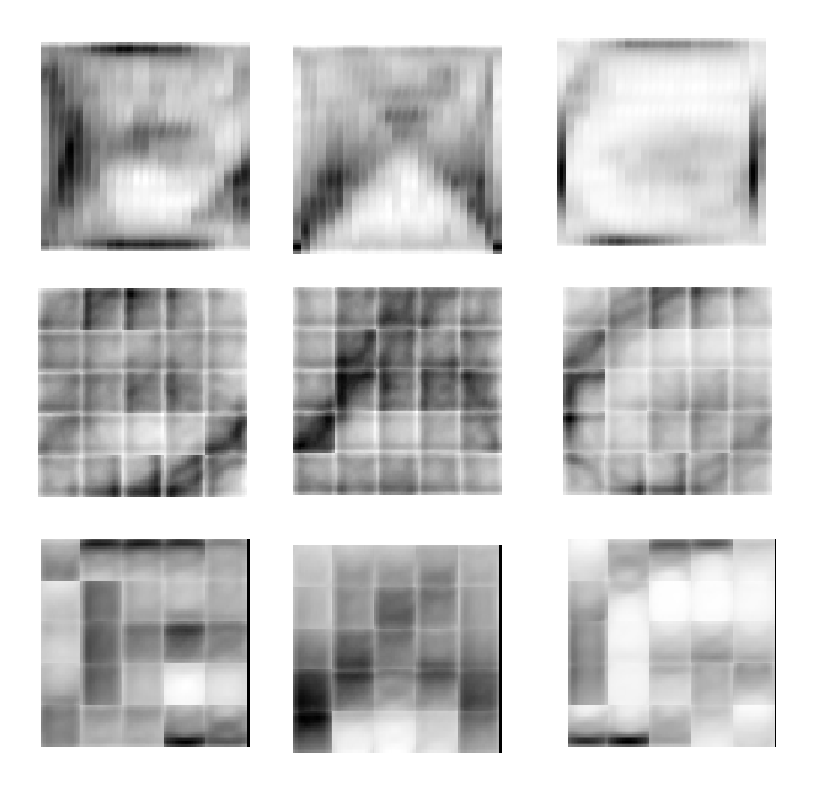
\includegraphics[width=10.0cm,height=10.0cm]{char}}
\end{minipage}
\caption{Character instances of B,A,G from HMMs. top row: DCT+strip, middle row: DCT+patch, bottom row: MB+patch}
\label{fig:chars}
\end{figure}

The generative models can be also to provide quantitative insight into the feature but also to compare the patch vs. strip sweep. By construction the transition matrices $\A$ is square with $\N_s$ states are diagonal dominant as we are forcing a inherent directionality through the way the image of the character is swept. The variance among the various handwritten characters are captured in the emission matrix ($\B$) which is a rectangular matrix of size $\N_s \times \N_l$ where $\N_l$ are number of emission labels at each state. In order to capture the variance efficiently matrix $\B$ has to be full-ranked. A low rank approximation of $\B$ was  performed to capture the emission probability at each state allowing an error of $10^{-6}$. In the current experiment $\N_s= 25$, $\N_l=20$, for an efficient feature the rank for the approximation matrix needs to be as high as possible $i.e$ as close to 20 as possible.

\begin{figure}[!t]
\begin{minipage}[b]{1.0\linewidth}
  \centering
  \centerline{\includegraphics[width=10.0cm,height=10.0cm]{rank}}
\end{minipage}
\caption{Reduced rank of emission matrices over various character HMMs}
\label{fig:rank}
\end{figure}

\section{Conclusions}
\label{sec:conc}
The HMMs performance of the ergodic and left-right topologies are almost identical over all the features. The naive strip feature suffers from fuzziness that arises in forgoing the orientation information in the image however resulting in a descriptive feature that does not require any prior clustering. The Marti-Bunke performs well when increasing the number of segments into which the image is divided into but suffers from performance issues when the sequence length get longer. Gabor feature outperform other features primarily due to the effectively handling the scaling that occurs over upper and lower case characters such as \emph{c,k,o,p,x}. The DCT feature is effective in encoding information in the lower frequency with performance at par with Gabor. The coefficients at various frequencies have some scaling information which results in a compact feature vector. In the handwriting community the sliding window technique could be improved by moving over to a patch based approach.

We would like to extend the current framework to incorporate other widely used features such as Scale Invariant Feature Transform, Histogram of Gradients etc. We would also like to compare various HMM topologies to enhance the performance further. The proposed experimental setup is quite simple and cane be used to compare various features that fall under HMM based transcription. In future testing the underlying restrictions of fixed state per character will be relaxed and the framework can help separate the learning HMMs training from that associated to feature learning.

\section{Acknowledgement}
\label{sec:ackno}
The authors would like to thank Alicia Fornes and Computer Vision Center at Universitat Autonoma de Barcelona for their help in extracting the character images from the NIST data-set. The research is funded by "Vetenskapsr\r{a}det grant 2012-5743" and the "q2b -- From Quill 2 Bytes initiative at Uppsala University".

\nocite{bal:cha:gra:pae}
\bibliographystyle{splncs}
\bibliography{isvc}

\end{document}
